\documentclass[12pt,letterpaper]{article}
\usepackage{amsmath, xparse}
\usepackage{graphicx}
\graphicspath{{/}}
\title{HW1}
\author{ZONGQI CUI}
\begin{document}
\section{}
    \begin{itemize}
    
        \item[Problem 1]\par
        \begin{itemize}
            
            \item[1(a)] $$\begin{aligned}
                T(n)&=2*T(n/2)+O(nlgn)\\
                &=2*(2*T(n/4)+O(n/2*lg(n/2)))+O(nlgn)\\
                &=2^2T(n/2^2)+O(nlg(n/2))+O(nlgn)\\
                &=2^3T(n/2^3)+O(nlg(n/4))+O(nlg(n/2))+O(nlgn)\\
                &\dots\\
                &=2^kT(n/2^k)+O(nlg(n/2^{k-1}))+\dots+O(nlg(n/2))+O(nlgn)
                \end{aligned}$$
                
                Since we need to divide the original problem into a minimum size, so $n/2^k =1$, which is, $n=2^k, k=lgn$.  And $T(1)=1$, we have,
                
                $$\begin{aligned}
                T(n) &= n+n(lg(2n/2^k)+lg(4n/2^k)+\dots+lg(n/2)+lgn)\\
                &= n+n(lg2+lg4+\dots+lgn-1+lgn)\\
                &=n+n(1+2+3+\dots+lgn-1+lgn)\\
                &=n+n(lgn(lgn+1)/2)\\
                &=n+(nlg^2n+nlgn)/2\\
                &=O(nlg^2n)
                \end{aligned}$$
    
            \item[1(b)] 

            
            $$\begin{aligned}
                T(n)&=2*T(n/2)+O(n/lgn)\\
                &=2*(2*T(n/2^2)+O(n/2/lg(n/2)))+O(n/lgn)\\
                &=2^2T(n/2^2)+O(n/lg(n/2))+O(n/lgn)\\
                &=2^3T(n/2^3)+O(n/lg(n/4))+O(n/lg(n/2))+O(n/lgn)\\
                &\dots\\
                &=2^kT(n/2^k)+O(n/lg(n/2^{k-1}))+\dots+O(n/lg(n/2))+O(n/lgn)
                \end{aligned}$$
                
                The same as the previous question, we know that $n=2^k, k=lgn$. Therefore, using the same strategy, we have,
                
                $$\begin{aligned}
                T(n) &= n+n(1/lg2+1/lg4+\dots+1/(lgn-1)+1/lgn)\\
                &= n+nlg(lgn)\\
                &= O(nlglgn)
                \end{aligned}$$
            \item[1(c)] 
            $$\begin{aligned}
                T(n) &= \sqrt{n}T(\sqrt{n})+O(n)\\
                &=n^{\frac{1}{2}}(n^{\frac{1}{4}}T(n^{\frac{1}{4}})+O(\sqrt{n}))+O(n)\\
                &=n^{\frac{1}{2}+\frac{1}{4}}T(n^{\frac{1}{4}})+2n\\
                &=n^{\frac{1}{2}+\frac{1}{4}+\frac{1}{8}}T(n^{\frac{1}{8}})+3n\\
                &\dots\\
                &=n^{\sum_{i=1}^k\frac{1}{2^i}}T(n^{\frac{1}{2^k}})+kn
                \end{aligned}$$
                
                As $T(1)=1$, and obviously the original problem cannot be divided into subproblems of size 1, which can cause $n=1$, so we assume T(2)=2, which is reasonable, and we have
                
                $$\begin{aligned}
                n^{\frac{1}{2^k}}&=2\\
                \frac{1}{2^k}lgn&=1\\
                k&=lglgn
                \end{aligned}$$
                
                Substituting k into T(n), we have
                
                $$\begin{aligned}
                T(n)&=2n^{\sum_{i=1}^{lglgn}\frac{1}{2^i}}+nlglgn\\
                &=2n^{1-\frac{1}{lgn}}+nlglgn\\
                &=O(nlglgn)
            \end{aligned}$$
            \item[1(d)]
            The original problem is,

            $$\begin{aligned}
            T(n)&=T(n/4)+T(n/2)+O(n),
            \end{aligned}$$

            and we can expand the equation like a recursive tree, and the cost for the first layer is $n$, the cost for the second layer is $\frac{3}{4}n$, that is, $\frac{1}{4}+\frac{1}{2}$, and the third layer is $\frac{9}{16}n$,which is $(\frac{3}{4})^2n$. And in order to divide the problem into a subproblem of size 1, there're supposed to be $log_4^n$ layers. Therefore, the total cost of the original problem is,

            $$\begin{aligned}
            T(n)&=n+\frac{3}{4}n+(\frac{3}{4})^2n+(\frac{3}{4})^3n+\dots+(\frac{3}{4})^{log_4^n}n\\
            &=n*(\frac{1-(\frac{3}{4})^{log_4^n}}{1-\frac{3}{4}})\\
            &=O(n)
            \end{aligned}$$
             
        \end{itemize}

        \item[Problem 2]\par
        \begin{itemize}
            \item[2(a)]\par
            answer:\par
                A matrix is invertible if and only if its determinant is not zero. 
                A key property of Fourier transform matrices is that 
                if $\omega $ is a primitive unit root, then its rows (or columns) are 
                orthogonal and therefore linearly independent, which ensures that 
                the matrix is invertible.\par
                However, if $\omega^k$ for some smaller $k$, 
                it means that the powers of $\omega $ repeat before reaching $n $,
                leading to a situation where the rows (or columns) of the matrix are not all linearly independent. 
                This linear dependence implies that the determinant is zero, 
                so the matrix is not invertible.
            \item[2(b)]\par
            answer:\par  
            n=4 and $\omega=i$\par
                $ M_n(\omega)=
                \begin{bmatrix}
                   1 & 1 & 1 & 1\\
                   1 & i & -1 & -i\\  
                   1 & -1 & 1 & -1\\ 
                   1 & -i & -1 & 1\\ 
                \end{bmatrix} $\par$ =
                \begin{bmatrix}
                    1 & 1 & 0 & 0\\
                    0 & 0 & 1 & 1\\  
                    1 & -1 & 0 & 0\\ 
                    0 & 0 & 1 & -1\\ 
                 \end{bmatrix}\times 
                 \begin{bmatrix}
                    1 & 0 & 1 & 0\\
                    0 & 1 & 0 & 1\\  
                    1 & 0 & -1 & 0\\ 
                    0 & i & 0 & -i\\ 
                 \end{bmatrix}
                 $
            \item[2(c)]\par
            answer:\par
            \begin{figure}[h]
                \centering
                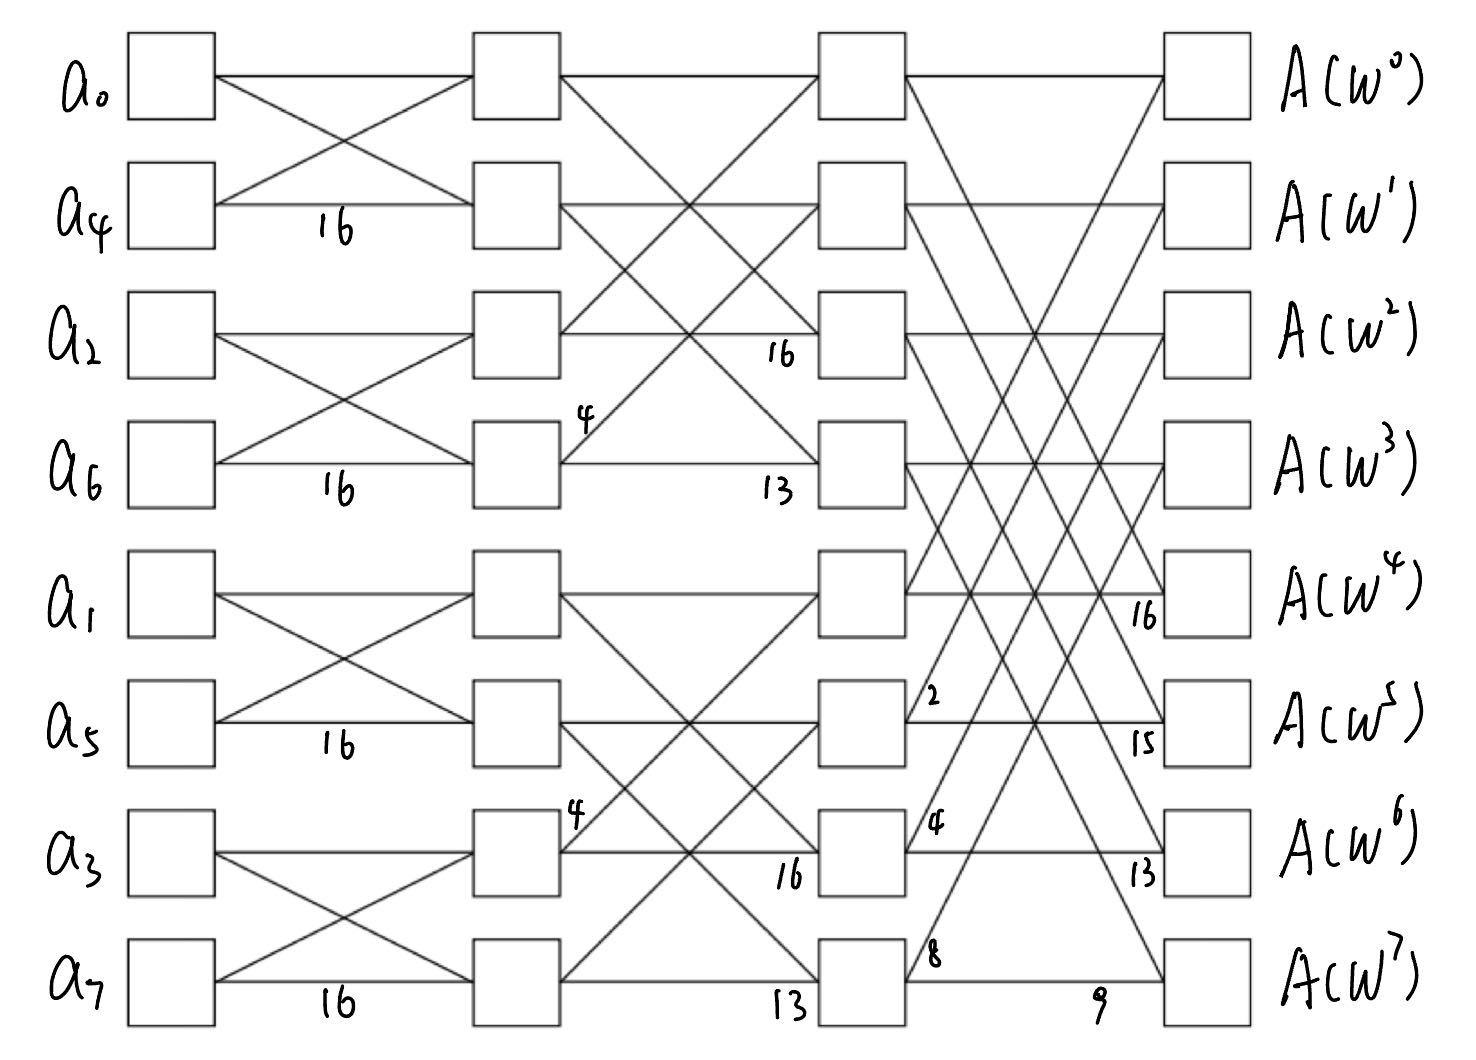
\includegraphics[scale=0.2]{butterfly.jpg}
                \caption{2(c)}
            \end{figure}
        \end{itemize}
        \item[Problem 3]\par
             answer:\par
            \begin{itemize}
                \item[(1).] if $n==1$ then $A(x)=x-r_1$
                \item[(2).] we split the set of roots into two halves:\[{r_1,r_2,\dots,r_{n/2}}\]and \[{r_{n/2+1},r_{n/2+2}+\dots+r_n}\]
                \item[(3).]  let \[A_1(x)={r_1,r_2,\dots,r_{n/2}}\] \[A_2(x)={r_{n/2+1},r_{n/2+2}+\dots+r_n}\]
                \item[(4).] compute $A_1(x)$ and $A_2(x)$ recursively
                \item[(5).] combine the result: \[A(x)=A_1(x) \times A_2(x)\] 
            \end{itemize}
            running time:
                \[T(n)=2T(n/2)+O(nlogn)\]
                we can get \[T(n)=O(nlog^2n)\]
        \item[Problem 4]\par
            answer:\par
            In the \textit{Fast Multipoint Evaluation On n Arbitrary Points}, the author uses two steps, multiplying up the tree and dividing down the tree and manage to control the runtime in $O(nlg^2n)$.

            For multiplying up the tree, let $u_0,\dots,u_{n-1}$ be given points in the ring $R$. The first step of the algorithm is to build a tree starting with the polynomial $x-u_i$ for $0\leq i < n$ as the leaves.Each node represents a polynomial that is constructed as the product of its children. The polynomial $M_{i,j}$ resides at height $i, j$ nodes from the left, and is the product of all the leaves that lay underneath it. The root of the tree represents $M{k,0}=\prod_{i=0}^{n-1}(x-u_i)$, and each leaf represents $M_{0,j}=x-u_j$.

            For dividing down the tree, let $R = \mathcal{Z}_p$ for $p$ a fourier prime. For $0\leq i < n$, let $m_i=x-u_i$, and define the canonical ring homomorphism

            $$\begin{aligned}
            \pi_i:R \implies R/\langle m_i \rangle,  \\
            \pi_i(f)=f \mod m_i.
            \end{aligned}$$

            We know the composition of ring homomorphisms is again a ring homomorphism, so
            $$\begin{aligned}
            \mathcal{X}=\pi_0 \times \pi_1 \times \dots \pi_{n-1}:R \implies R/\langle m_0 \rangle \times \langle m_1 \rangle \times \langle m_{n-1} \rangle, \\
            \mathcal{X}(f) = (f \mod m_0, \dots, f \mod m_{n-1}).
            \end{aligned}$$
            Notice that we chose the moduli in such a way that $f$ evaluated at $u_i$ is
            $$
            f(u_i)=q(u_i)m_i(u_i)+r(u_i)=r(u_i).
            $$

            This is equivalent to saying that $f(u_i) = f(x) \mod (x-u_i)$. Since $f \mod m_i$ must have degree less than the degree of $m_i$, and each $m_i$ is linear, it follows that $f \mod m_i \in \mathcal{R}.$ Therefore,

            $$\begin{aligned}
            \mathcal{X}=:R \implies R/\langle m_0 \rangle \times \langle m_1 \rangle \times \langle m_{n-1} \rangle,\\
            \mathcal{X}(f) = (f(u_1), \dots, f(u_{n-1})).
            \end{aligned}$$

            We now have a method for evaluating a polynomial at $n$ points. However, dividing a polynomial of degree $n-1$ by $n$ linear polynomials is still $O(n^2)$, as each division requires $n$ multiplications in the ring. We can save work by performing larger divisions rather than $n$ linear divisions. Instead of dividing $f$ by the leaves of the tree, we will recurse down the tree. First, let
            
            \[r_0=f\mod \prod_{i=0}^{n/2-1}(x-u_i)=M_{k-1,0}\]  
            \[r_1=f\mod\prod_{i=n/2}^{n-1}(x-u_i)=M_{k-1,1}\].
            
            Then, call the algorithm on inputs $r_0, n/2$ and the subtree rooted at $M_{k-1,0}$ and again on inputs $r_1, n/2$ and the subtree rooted at $M_{k-1,1}$. Since the subproduct tree is a binary tree of height $lgn$, we will reduce the number of polynomial divisions required to compute an evaluation to $O(lgn)$.
        \item[Problem 5]
            answer:\par
            \begin{itemize}
                \item [(1).]\textbf{base case}:\par If subgraph is smaller than 10 vertices, we can simply get results by DFS(Depth-First Search)  
                \item [(2).]we can randomly select 9 vertices in the middle of the graph,and we split graph into two parts:
                                \begin{itemize}
                                    \item left part: vertice index lower than the separator
                                    \item right part:vertice index higher than the separator
                                \end{itemize}
                            compute these two parts recursively
                \item [(3).]combine the both parts results,including all of the separator vertices and make sure no adjacent vertices in the left or right are included.
            \end{itemize}
    \end{itemize}
    

    
\end{document}